\documentclass[conference]{IEEEtran}
\usepackage{amsmath,amssymb,amsfonts}
\usepackage{algorithm2e}
\usepackage[noend]{algpseudocode}
\usepackage{graphicx}
\usepackage{textcomp}
\usepackage{xcolor}
\usepackage[english]{babel}
\usepackage[utf8]{inputenc}
\usepackage[nottoc]{tocbibind}
\usepackage{natbib}
\usepackage{graphicx}
\graphicspath{ {./images/} }

\begin{document}

\title{COS710: Assignment 2}

\author{\IEEEauthorblockN{Myron Guanhao Ouyang}
\IEEEauthorblockA{\textit{Department of Computer Science} \\
\textit{University of Pretoria}\\
South Africa \\
u16008368@tuks.co.za}
}
\maketitle

\begin{abstract}
    This paper demonstrates that the Ant Colony Optimization (ACO) algorithm is superior in terms of performance when compared to the Beam Search (BS) algorithm. Performance in this paper is based on the each algorithms ability to find the longest path in a series of mazes (of varying sizes and complexity) in the shortest time span. ACO is able to consistently find paths through the maze that is longer than that found by BS.
\end{abstract}


\section{Introduction}
    The primary objective of this paper is to compare the performance between the Ant Colony Optimization (ACO) algorithm and the Beam Search (BS) algorithm.
    
    ACO or Simple Ant Colony Optimization (SACO) is an improvement, developed by Gambardella and Dorigo \cite{Slides1}, to the performance of the base Ant System (AS).
    
    Beam Search, also known as Best First Search, is in essence an alteration on the classic Breadth First Search by adding a heuristic aspect (a priority queue) to the search itself.
    
    The paper follows the following format; Section II will be a high level discussion on the approaches used for both algorithms. Section III will be a more in depth view of the algorithms, Section IV will show the results of the implementation of both algorithms and finally Section V will conclude the results of this paper.
\section{Background}
    The background section will give a brief history of the AS and a high level overview of both algorithms.
    
    Ant algorithms are aptly named as they are modeled after the insect itself. It attempts to copy how ants are capable of communicating with one another without the need to know the position of each other. Ants are able to do this through the use of pheromone trails \cite{Slides1}. It is this aspect of indirect communication between entities that the Ant algorithm attempts to mimic.
    
    \subsection{Maze Background}
        The code and algorithm to convert the maze from a picture format into a traversable Maze Class format was adapted and modified from open source code provided by Michael Pound \cite{Mazecode}. Modification to the base code include; calculating distance between nodes and changing node neighbours to include a pheromone attribute. 
    \subsection{ACO Background}
        ACO was developed as an improvement on the standard AS's performance, by modifying the node choosing process to include heuristic information and also including some stochasticity in the decision making process. 
        If Ant $k$ is currently located at node $i$, the rule to select the next node $j$ is defined as follows:
        \begin{equation}
            j= 
              \begin{cases}
              \mathit{argmax}_{u\epsilon\mathit{N_{i}^{k}(t)}}\tau_{i,u}(t)\eta_{i,u}^{\beta}(t)   & \text{if } r \leq r_{0} \\
              J,             & \text{if } r > r_{0}
              \end{cases}\\
        \end{equation}
        where $r \sim U(0,1)$ and $r_0 \in [0,1]$ is user defined \\
        $J \in \mathcal{N}_i^k(t)$ is a randomly selected node according to the following probability:
        \begin{equation}
            P_{i,J}^k = \frac{
                \tau_{i,J}^\alpha(t)\eta_{i,j}^\beta(t) 
            }{
                \sum_{u,\in,\mathcal{N}_i^k}\tau_{i,u}^\alpha\eta_{i,u}^\beta(t)
            } \text{if } j \in \mathcal{N}_{i}^{k}\\
        \end{equation}
        Once a node has been selected, the path (or Edge) between the nodes has its pheromone attribute updated. This is known as the Local Update and is defined as follows:
        \begin{equation}
            \tau_{i,j}(t) = (1 - \rho_2)\tau_{i,j}(t) + \rho_2\tau_0 
        \end{equation}
        with $\rho_2$ being the local evapouration factor.
        Once all ants have completed the maze, a global pheromone update is applied to each Ant's path, it is defined as follows:
        \begin{equation}
            \tau_{i,j}(t) = (1 - \rho_1)\tau_{i,j}(t) + \rho_1\triangle\tau_{i,j}(t)
        \end{equation}
        where:
        \begin{equation}
            \triangle\tau_{i,j}(t) = 
            \begin{cases}
              \frac{Q}{f(\hat{x}(t)}  & \text{if link (i, j) occurs in $\hat{x}$(t)}  \\
              0,             & \text{Otherwise }
              \end{cases}\\
        \end{equation}
        and the Best Path $\hat{x}(t)$ is determined either after every successful iteration $t$ or after every epoch.
        $Q$ is a positive user defined constant and the function $f(\hat{x}(t))$ is a user defined heuristic.
        
        Below is a basic Pseudo code for an Ant traversing a maze:
        
        \begin{algorithm}[H]
            \caption{Pseudo code for Ant}
            \SetAlgoLined
            \SetKwProg{Def}{def}{:}{}
            \Def{run(bestPath)}{
                \Repeat{Forever}{
                    \If{$currentPosition == end.Position$}{
                        break
                    }
                    $neighbours = currentNode.GetAvailableNeighbours()$ \newline
                    \uIf{$neighbours == Empty$}{
                        $backtrack()$
                    }
                    \Else{
                        $currentPosition = chooseNextNode(neighbours)$ \\
                        $localUpdatePheromone()$ \\
                        $updateVisitedList()$ \\
                        $updatePathList()$ \\
                    }
                }
                $globalUpdatePheromone(bestPath)$\\
                return $PathList$\;
            }
        \end{algorithm}
        The following is a basic implementation of the ACO solve function:
        \begin{algorithm}[h]
            \caption{Pseudo code for ACO}
            \SetAlgoLined
            \SetKwProg{Def}{def}{:}{}
            \Def{solve()}{
                bestPath = $Null$ \\
                bestDistance = 0 \\
                \For{epoch}{
                    \For{TotalAnts}{
                        ant = Ant()\\
                        result =  ant.run(bestPath)\\
                        \If{$result.distance > bestDistance$}{
                            bestPath = result \\
                            bestDistance = result.distance
                        }
                        
                    }
                }
                return $bestPath$\;
            }
        \end{algorithm}
    \subsection{BS Background}
        The Beam Search implementation is relatively similar to that of the normal Breadth First Search (BFS) with only minor alterations. The first being the introduction of a Priority Queue and the Beam Width parameter. The Priority Queue differs from the normal Queue data structure that the BFS uses in the the way that elements in the queue are reordered based on their heuristic value. The size of the Queue is also limited to the Beam Width.  
        
\section{Implementation}
    This section describes, in detail, the steps and thought processes followed to implement the three algorithms.
    \subsection{Maze Implementation}
        As mentioned in the previous section, the primary logic of the algorithm has been unchanged. The only alterations made were; ensuring the edge between nodes had a $Pheromone$ attribute that was initialized to 1 and also included a distance attribute.
        The algorithm converts the image of a maze into a workable list of nodes. Each node has a maximum of 4 neighbours and is only created if its corresponding position on the maze is on a junction (path is available on both x and y axis), it has reached the end of a path or it is either the start or end of the maze.
        \begin{figure}[h]
        \centering
        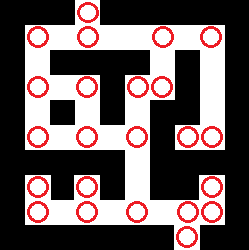
\includegraphics[width=0.3\textwidth]{maze_grid}
        \caption{10x10 Maze}
        \end{figure}
    \subsection{ACO Implementation}
        The ACO user defined constants used in this assignment are as follows:
        \begin{align}
           & \alpha = 1\\
           & \beta = 3 \\
           & p_2 = 0.1 \\
           & p_1= 0.6 \\
           & r_0 = 0.9 \\
           & Q = 2 \\
           & numAnts = 5 \\
           & epochs = 3
        \end{align}
        To optimize the efficiency of the ants while they are traversing the maze, if the ant needs to backtrack because it has hit a dead end, whilst backtracking they set the pheromone level on the connecting edge to $0.01$ to ensure no future ant will take the path that leads to a dead end. In an attempt to further optimize efficiency of the algorithm, each ant is coded as its own separate thread; hence allowing concurrent traversal of the maze.
        The heuristic $\eta$ used is relatively simple and is calculated as follows:
        \begin{equation}
            \eta = 
            \begin{cases}
              distance  & \text{if moving up}  \\
              distance * 0.5  & \text{if moving down}  \\
              distance * 0.75      & \text{if moving left or right}  \\
              \end{cases}\\
        \end{equation}
        This simply gave a slight bias for the ant to explore around the maze, avoiding the exit for as long as possible, hence giving a higher chance of finding the longer path.
        
        The function $f(\hat{x}(t))$ is used to determine the quality of the path compared to the currently best path $\hat{x}$. It is calculated as follows:
        \begin{equation}
            currentDistance / bestDistance
        \end{equation}
        
        Finally, in this implementation of ACO, a $Global-Best$ approach was taken to decide the $\hat{x}$, meaning the $\hat{x}$ was only decided after every epoch.
    \subsection{BS Implementation}
        The user defined constants used in the Beam Search are as follows:
        \begin{align}
           & beamWidth = \text{Width of Maze}
        \end{align}
        The heuristic used to order the priority queue is the same as the one used in ACO, equation 14.
\section{Research Results}
    This sections serves as a summary of the research results for both algorithms and what observations can be made.
    \subsection{ACO Results}
        Table 1 shows the longest path found and the time it took the ACO to find the path for the various maze sizes.
        Figures 2, 3 and 4 show completed mazes using the ACO algorithm.
\begin{table}[h]
\begin{tabular}{|l|r|r|}
\hline
\textbf{Maze Name}      & \multicolumn{1}{l|}{\textbf{Distance (pixel)}} & \multicolumn{1}{l|}{\textbf{Time (min)}} \\ \hline
\textbf{Small 1}        & 248                                            & \textless 1                              \\ \hline
\textbf{Small 2}        & 76                                             & \textless 1                              \\ \hline
\textbf{Small-Medium 1} & 4580                                           & \textless 1                              \\ \hline
\textbf{Small-Medium 2} & 1888                                           & \textless 1                              \\ \hline
\textbf{Small-Medium 3} & 2432                                           & \textless 1                              \\ \hline
\textbf{Small-Medium 4} & 269                                            & \textless 1                              \\ \hline
\textbf{Medium 1}       & 241454                                         & $\sim$2                                 \\ \hline
\textbf{Medium 2}       & 132488                                         & $\sim$2                                 \\ \hline
\textbf{Medium 3}       & 14379                                          & $\sim$3                                  \\ \hline
\textbf{Large 1}        & 2911982                                        & $\sim$20                                    \\ \hline
\end{tabular}
\caption{Results for ACO}
\label{ACO}
\end{table}
        \begin{figure}[H]
            \centering
            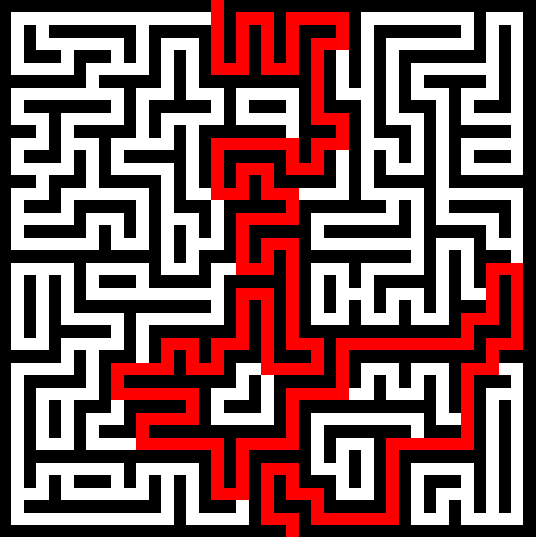
\includegraphics[width=5cm]{images/ACO_Small1.png}
            \caption{ACO Solution Small 1}
            \label{ACO_Small1}
        \end{figure}
        \begin{figure}[H]
            \centering
            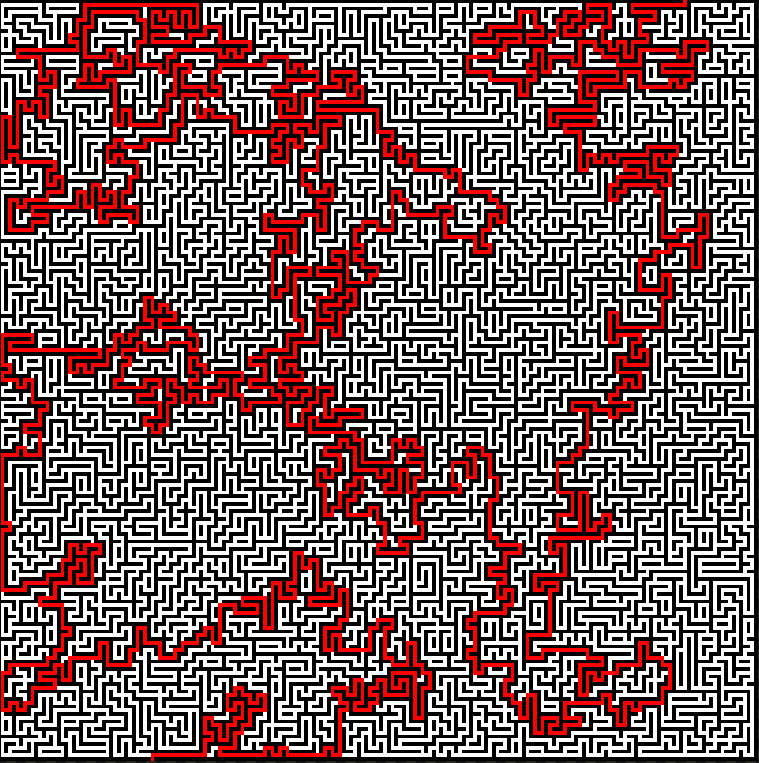
\includegraphics[width=5cm]{images/ACO_SM1.png}
            \caption{ACO Solution Small-Medium 1}
            \label{ACO_SM1}
        \end{figure}
        \begin{figure}[H]
            \centering
            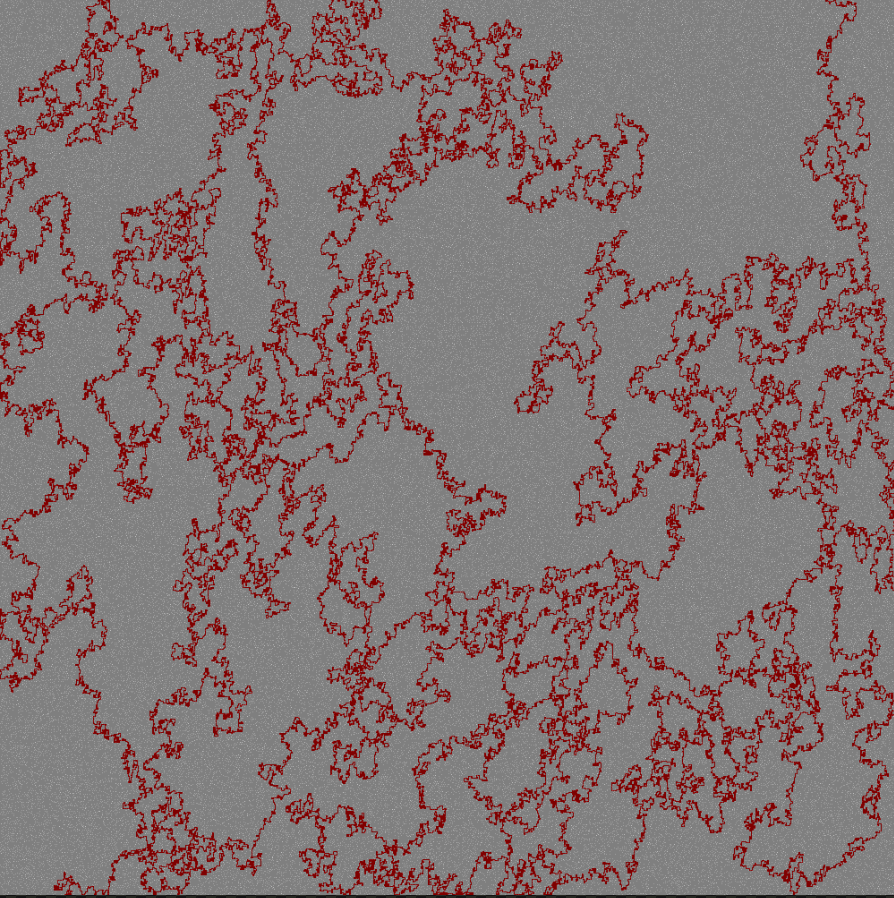
\includegraphics[width=5cm]{images/ACO_M1.png}
            \caption{ACO Solution Medium 1}
            \label{ACO_M1}
        \end{figure}
    \subsection{BS Results}
        Table 2 shows the longest path found and the time it took the Beam Search to find the path for the various maze sizes.
        Figures 5, 6 and 7 show completed mazes using the BS algorithm.

\begin{table}[h]
\begin{tabular}{|l|r|r|}
\hline
\textbf{Maze Name}      & \multicolumn{1}{l|}{\textbf{Distance (pixel)}} & \multicolumn{1}{l|}{\textbf{Time (min)}} \\ \hline
\textbf{Small 1}        & 141                                            & \textless 1                              \\ \hline
\textbf{Small 2}        & 77                                             & \textless 1                              \\ \hline
\textbf{Small-Medium 1} & 989                                            & \textless 1                              \\ \hline
\textbf{Small-Medium 2} & 1005                                           & \textless 1                              \\ \hline
\textbf{Small-Medium 3} & 2433                                           & \textless 1                              \\ \hline
\textbf{Small-Medium 4} & 269                                            & \textless 1                              \\ \hline
\textbf{Medium 1}       & 21091                                          & $\sim$2                                  \\ \hline
\textbf{Medium 2}       & 19645                                          & $\sim$1                                  \\ \hline
\textbf{Medium 3}       & 14379                                          & \textless 1                              \\ \hline
\textbf{Large 1}        & 91071                                          & $\sim$250                                \\ \hline
\end{tabular}
\caption{Results for BS}
\label{BS}
\end{table}
    \begin{figure}[h]
        \centering
        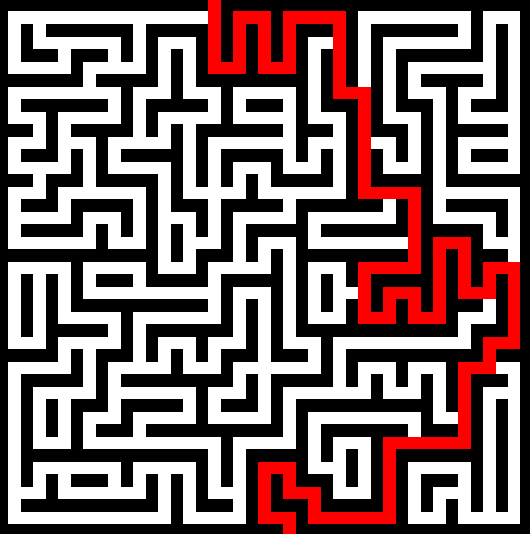
\includegraphics[width=5cm]{images/BS_Small1.png}
        \caption{BS Solution Small 1}
    \end{figure}
    \begin{figure}[h]
        \centering
        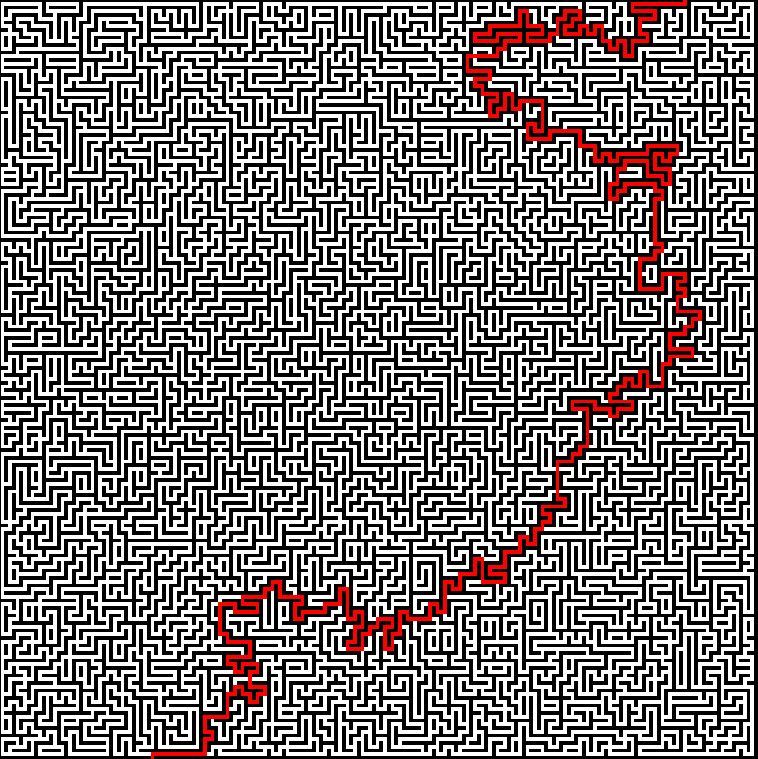
\includegraphics[width=5cm]{images/BS_SM1.png}
        \caption{BS Solution Small-Medium 1}
    \end{figure}
    \begin{figure}[h]
        \centering
        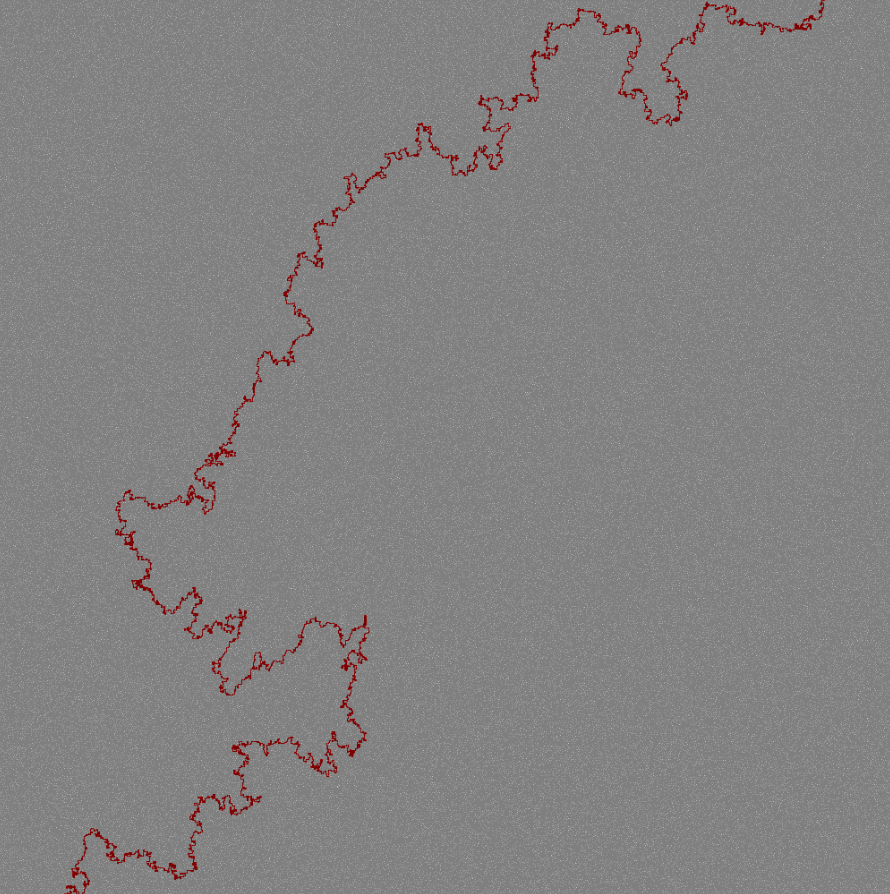
\includegraphics[width=5cm]{images/BS_M1.png}
        \caption{BS Solution Medium 1}
    \end{figure}
    \subsection{Observations}
        It is clear from the above tables that, in terms of performance, ACO is far better than BS. It seems that BS is appropriate for situations in which there is only one acceptable outcome, as it was able to reach the conclusion faster than ACO. Evidence in results regarding Small 2, Small-Medium 4 and Medium 3. 
        
        However that is to be expected as the nature of an ACO algorithm is to explore. The results (namely the distance) of the ACO algorithm varies slightly due to its stochasticity  however in this experiment it was always equal to or greater than that of the BS. BS lacking any randomness will always produce the same results no matter how many runs or epochs. 
        
        If a different heuristic is applied to BS, it may yeild better results. 
\section{Conclusion}
    From the results obtained in the previous section, ACO seems to be far superior to the BS in terms of both time to complete and maximum distance obtained. The additional complexity of ACO compared to BS is justified by the results.
    

\bibliographystyle{unsrt}
\bibliography{mybib}

\appendix
    
    
\end{document}
